% Session 1 -- the exponential wall: one matrix versus a Fock space.
% Placement: sec. "Where the two formalisms diverge", after the three-site paragraph.
% Rendered by figures/blender/s01f01_fockspace.py, labels in figures/overlays/s01f01_fockspace.tex.
\begin{aqmfigure}{fig:s01:fockspace}{The exponential growth of the Fock space for three sites. A
single-particle tight-binding problem is an $L\times L$ matrix, on the left, where the raised dark
entries are the first-neighbor hoppings of the chain in front of it. The interacting problem needs
the full Fock space, on the right, where every site is empty or occupied. Each plate is one
many-body state with a ball on every occupied site, and the $2^L$ states are ordered in columns by
particle number. For $L=3$ this is $8$, and for $L\approx20$ it is already about a million, which is
the limit of brute-force diagonalization.}
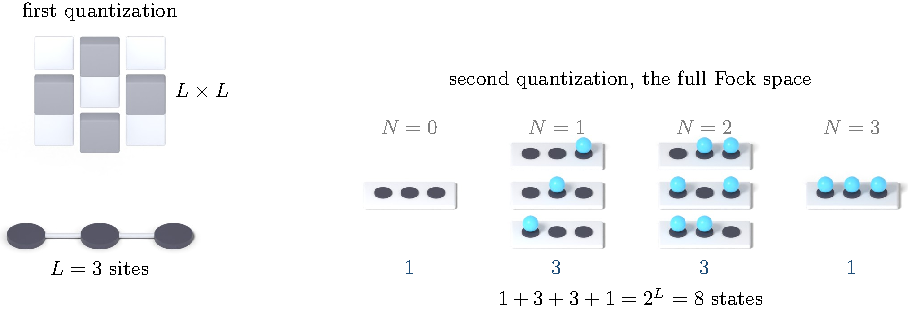
\includegraphics{figures/pdf/s01f01_fockspace.pdf}
\end{aqmfigure}
